\newcommand{\h}{$h(\vec{x})$}
\newcommand{\e}{\epsilon}
\chapter{Neural networks}\label{chapter:NN}



\section{The ROC curve and the optimal classifier}
One of the most common problem in machine learning is a binary classification, when a data set has to be divided into two subsets, fulfiling serian requirements. A simple example of such a problem is distinction between signal and bacground events in deta collected by experiment. We would like to have a function which takes as agruments set of physical observables (eg. particles' energy, momentum, coordinates of vertexes), represents by $\vec{x}$ and returns sigle number. More formally, a clasyfier can be call any function $h: \vec x \rightarrow \mathbb{R}$ designed in such a way, that high \h values correspond signal events and low \h values correspond background event. In most cases a classyfier output is squeezed by activation function to some finate range, for example from 0 to 1. A threshold value  \h =c, which is the value separating signal and backgrond events is called a working point, and has to be set by a user. The signal efficiency will be defined as $\e_S=\int d\vec x \rho_S(\vec x) \Theta(h(\vec x) -c)$ and respectively a background efficiency $\e_B=\int d\vec x \rho_B(\vec x) \Theta(h(\vec x) -c)$.

Problems: how to represent a clasyfier performence, how to compare different clasyfiers and how to choose proper working point have been discused since many years. During World War II engeeners faced a probelm of a radar detection efficiency. With an increasing radar sensitivity a chance to detect an enemy aircraft increses. However, the chanse that signal is a fake caused by birds or other circumstances also increases. To represent this relation a so-colled ROC (\textbf{R}eceiver \textbf{O}perating \textbf{C}haracteristic curve) curve was invited. One axis represents a true positive rate  or a detection efficiency, second axis shows a background reduction. Each point on the curve represents working-point for the clasyfier. Comparing two different classyfiers someone can not compare performance for one working point, but has to compare all. Graphic reprezentation of compared classyficators can be given by ROC curves.

\begin{figure}[hb]
  \centering
  %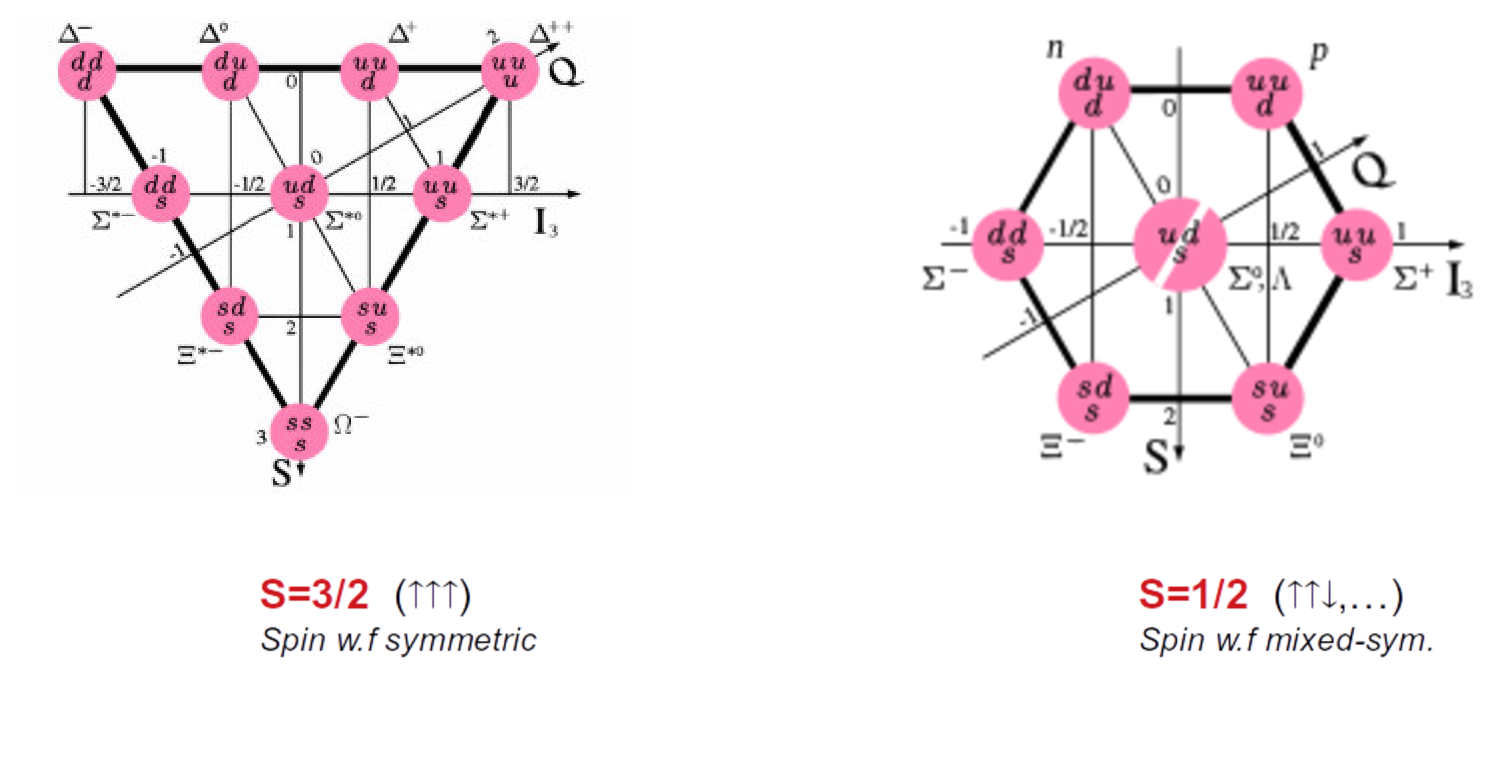
\includegraphics[width=0.9 \linewidth]{Chapter_introduction/eightfolds.eps}
  \caption{The ROC curve, it represents a clasyfier performence. In case of the ideal clasyfier area under the curve is equal 1, what means that for each working point all background events are rejected and non of singal is lost. }
  \label{fig:ROC}
\end{figure}

The optimal clasyfier is deffined as
\begin{equation}
  \forall c \forall \e_S
\end{equation}

In graphical approach the ptimal classyfier should give the biggest area under the ROC curve from all possible classyfiers. In case of complitly separable sets of data the area should be equal 1.
\section{The data-driven approach}
The original paper by Metodiev, Nachman and Thaler \cite{Metodiev_2017} the othors show the idea of a data-driven analysis in details. In this chapter I want to introduce main concepts, necessery to understand how the proposed metode helps in week decays recosntruction.

In a classical approach to supervized machine learning, a model learns its properties usign sets of labeled data. Of courese providing good training sets is always a problem. To do this, someone can use either experimental data, labeled by a user, or simulation. In first case a user uses his external knowledge about the data to describe it. In second case the user fully rely on simulation. First case is quite often impossible to perform, but even when a user is able to label data a labeling could be systematiclly biased by a lack of knowlage or missunderstand of detector. In second case they are two main threats: either a simulation does not describe data well, or creates some artificial structures in data, which can lead into sistematic errors in network performence. 

The data-data driven analysis avoids inconveniencees of two mentioned methodes. It requires neither labeling nor simulation and it bases only on statistical properties of a collected deta set. According to Neyman-Pearson lemma \cite{Neyman-Pearson} the optimal clasyfier for two sets, A and B is a function given by a dencity ratio
\begin{equation}
  \label{eq:N-P}
  h_{opt}^{A/B}(\vec x)=\frac{\rho_A}{\rho_B}
\end{equation}
or any monotonous function of $\frac{\rho_A}{\rho_B}$. Assuming that both sets A and B contains signal (s) and bacground (b) events and a statistical distribution of s and b is the same in A and B, we can write \eqref{eq:N-P} in the following way
\begin{equation}
  h^{A/B}_{opt}=\frac{f_1 \rho_s + (1-f_1) \rho_b}{f_2 \rho_s + (1-f_2) \rho_b}=\frac{f_1 \rho_s/\rho_b+1-f_1}{f_2 \rho_s/\rho_b+1-f_2}=\frac{f_1 h_{opt}^{s/b}+1-f_1}{f_2 h_{opt}^{s/b} +1-f_2}.
\end{equation}
It can be proven that $\partial_{h_{opt}^{s/b}}h_{opt}^{A/B} >0$, what means that optimal clasyfier for both cases is the same, so the clasyfier trained to distinguish A and B should also gives some separation power between signal and background. The situation is represented graphically in fig. \cite{fig:DD}.  It is important to underline that the reasoning gives no clue about the working points for both cases. 

\begin{figure}[h]
  \centering
  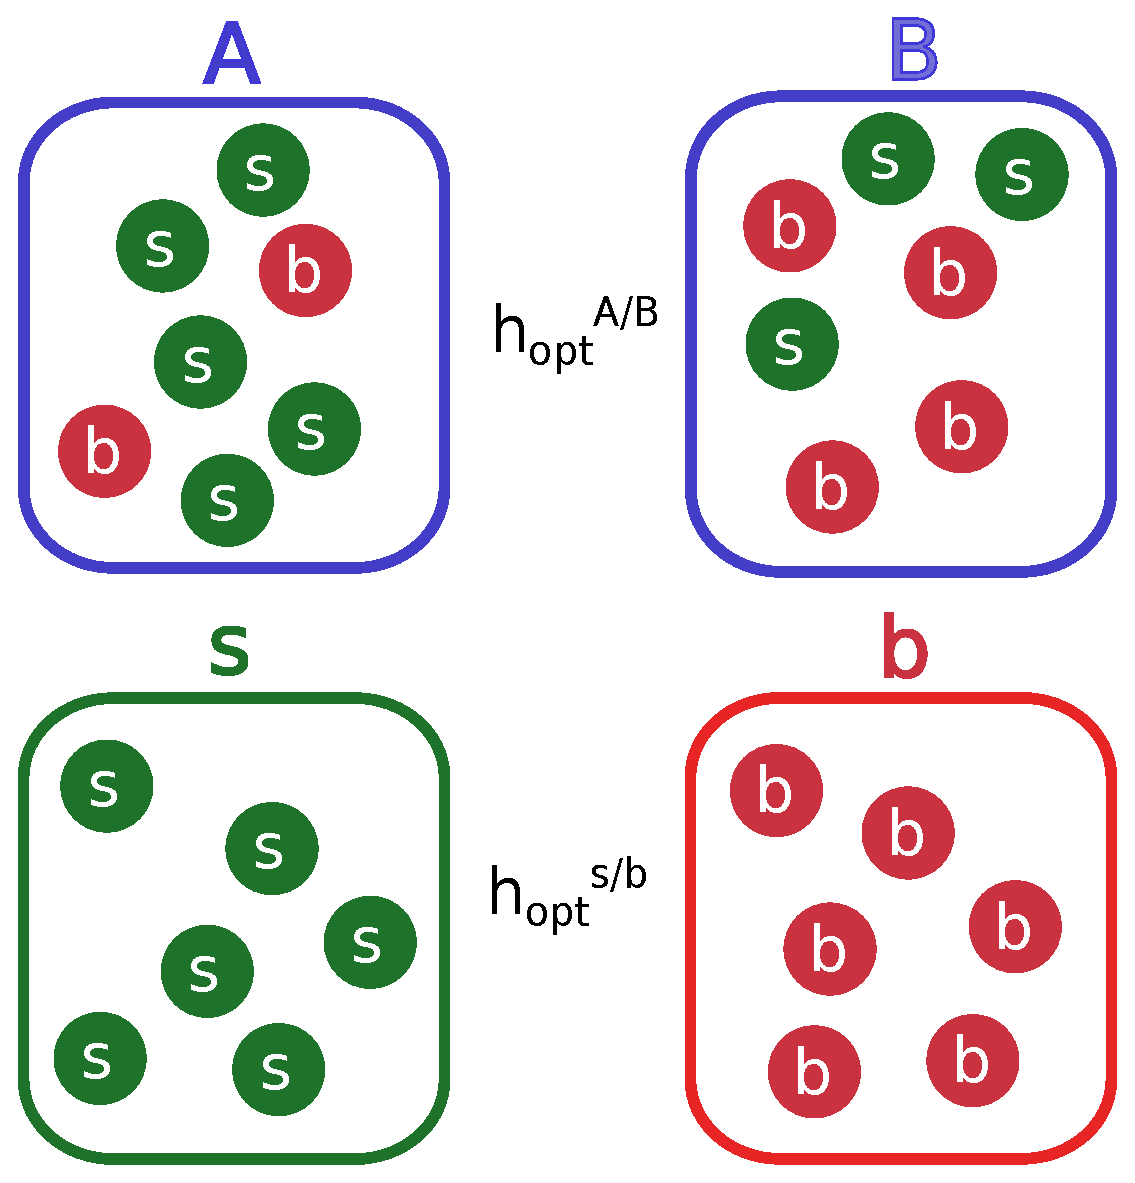
\includegraphics[width=0.5 \textwidth]{Chapter_NN/setAB.eps}
\caption{A data-driven approach visualisation. According to \cite{Metodiev_2017} the opitimal clasyfier for sets A and B is equivalent to optimal clasyfier for sets s and b.}
\label{fig:DD}
\end{figure}



\section{Application for analysis}
In case of $\Ls$ reconstruction the data driven approach was used to replace set of geometrical cuts and enchace a $\Lz$ signal~to~background ratio. So for the neural network all events with $\Lz$ were treated as a signal and without like a background. For all events an invariant mas of $\p \pim$ pair was ploted (fig. \ref{fig:L1116_DD}). Using this spectrun the dataset was divided in two subsets: for $M^{inv}_{\p\pim} \in (1015,1125)$ and $M^{inv}_{\p\pim} \notin (1015,1125)$. In the first of them a ratio between $\Lz$ and background is clearly different than in the second, what fulfil the requariments for the data-driven aproach. Hence, a numerous networka architecture were tested to check which deals the best with $\Lz$ reconstruction.

\begin{figure}[ht]
  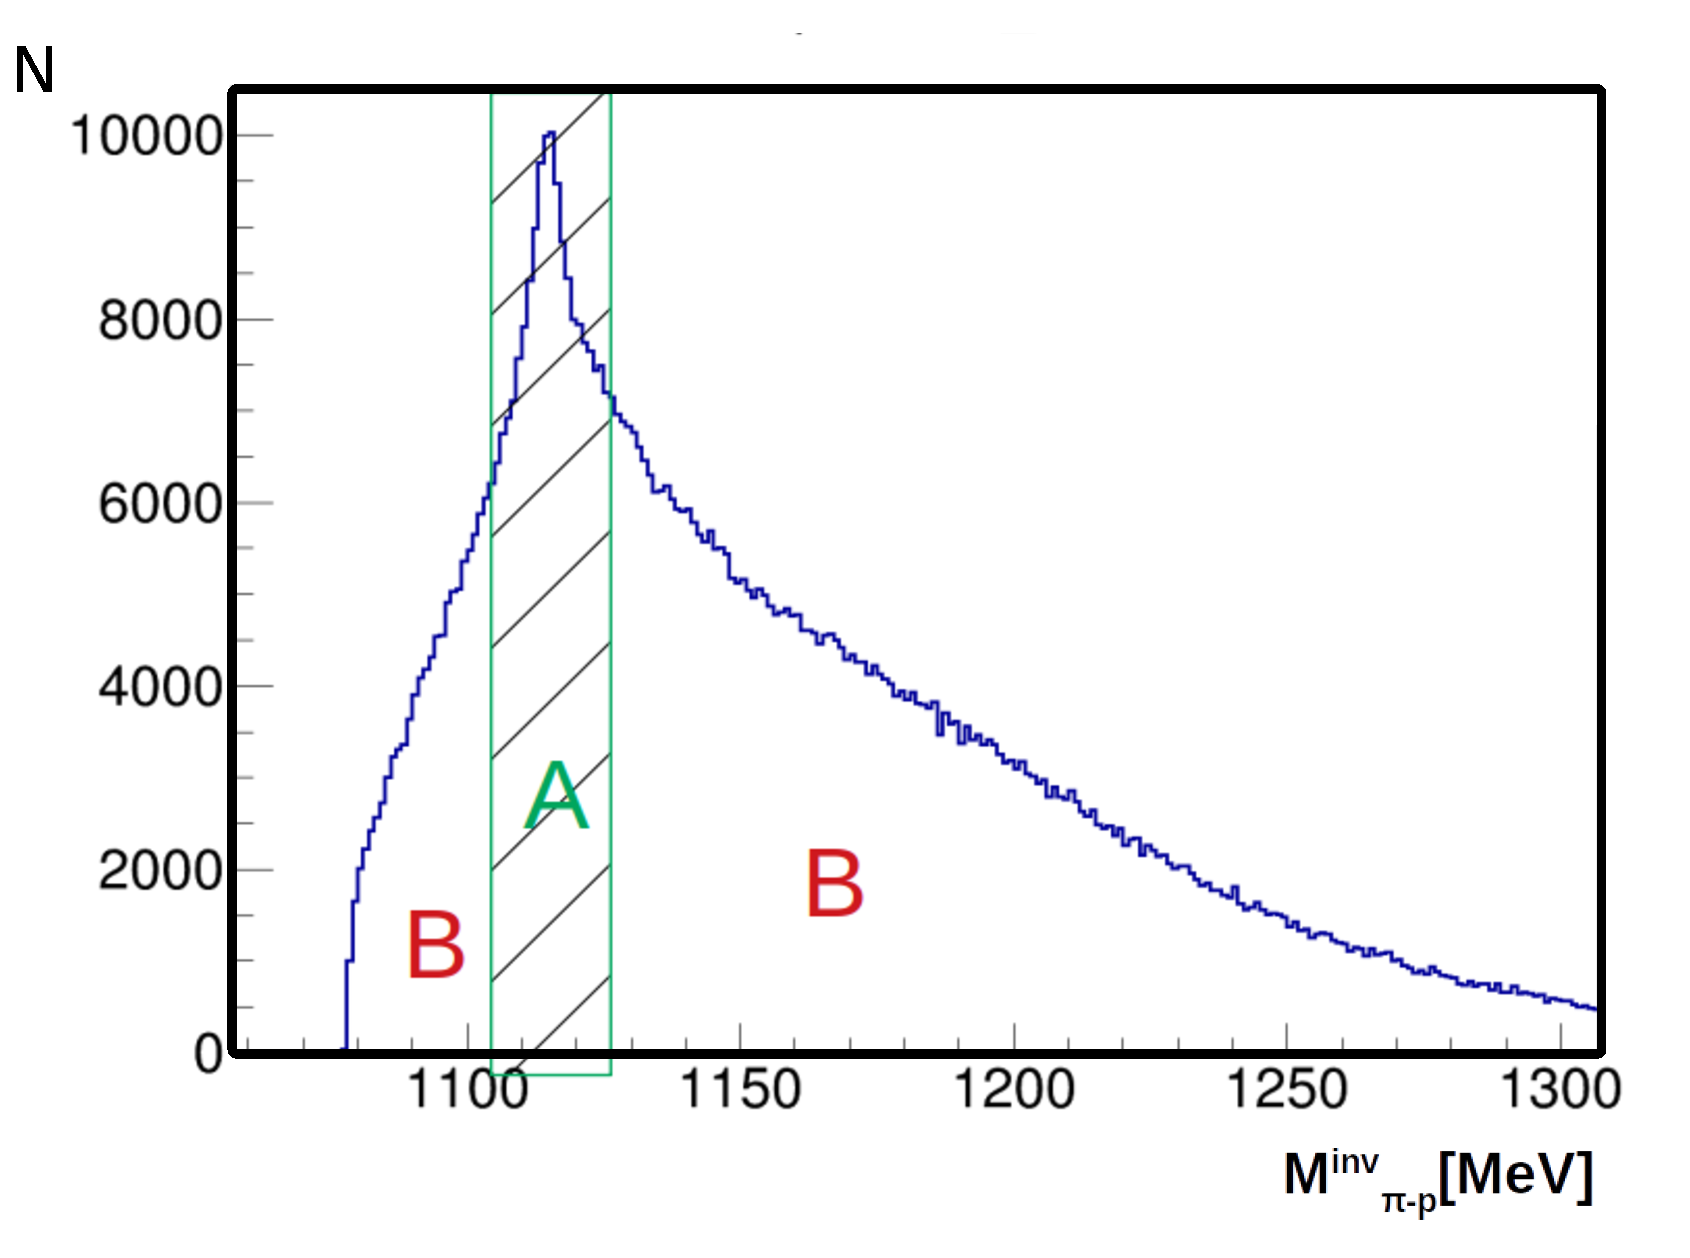
\includegraphics[width=0.8 \textwidth]{Chapter_NN/L1116.eps}
  \caption{A $\p \pim$ invariant mass specrum. Whole data set was divided into two subsets, A and B, each of them is characterized by different signal~to~background ratio. All tested models were trained to distinguish between sets A and B and later use to seperate events containing $\Lz$.}
  \label{fig:L1116_DD}
\end{figure}

A learning and testing proces was done within scope of TMVA framework \cite{TMVA}. Using TMVA a user has to provide list of input variables and a network architecture, than the framework automaticly preperes learning and testing sets and performs whole learning process together with testing the final classyfier. As an input variables the set of geometrical properties was used.
\begin{itemize}
\item Distance between $\p \pim$
\item $\Lz$ vertex cooridanes, reconstructed as a point of the closest aproach of $\p$ and $\pim$ tracks
\item $\Ls$ vertex coordinates, rseconstructed as a point of the closest approach of $\pip$ and $\pim$ tracks
\item $\Ls$ vertex coordinates, reconstructed by tracking algorithm as a primary vertex
\item Opaning angle between reconstructed $\Lz$ vector and a line conecting primary and secondary verteces
\end{itemize}
Using any combination of input variables it is impossile to reconstruct $\p \pim$ invariant mass. It is important feature wich allows to use mesioned invariant mass spectrum as a cross-check for all procedure, and a network will not collapse into trivial solution.

During treaning the network is optymalized to seperate sets A and B. Its performence for $\Lz$ reconstruction has to be investigated in a different way. After the traning the network was used to evaluate each event collected during the experiment. It means, that network output - a number in range from 0 to 1 - is assigned to each reconstructed event. Fitting a $\Lz$ peak (see \ref{fig:NN_wynik} a)) it was possible to check how signal efficiency and signal~to~background ratio changes with cut on the network output.

\begin{figure}[ht]
  \centering
  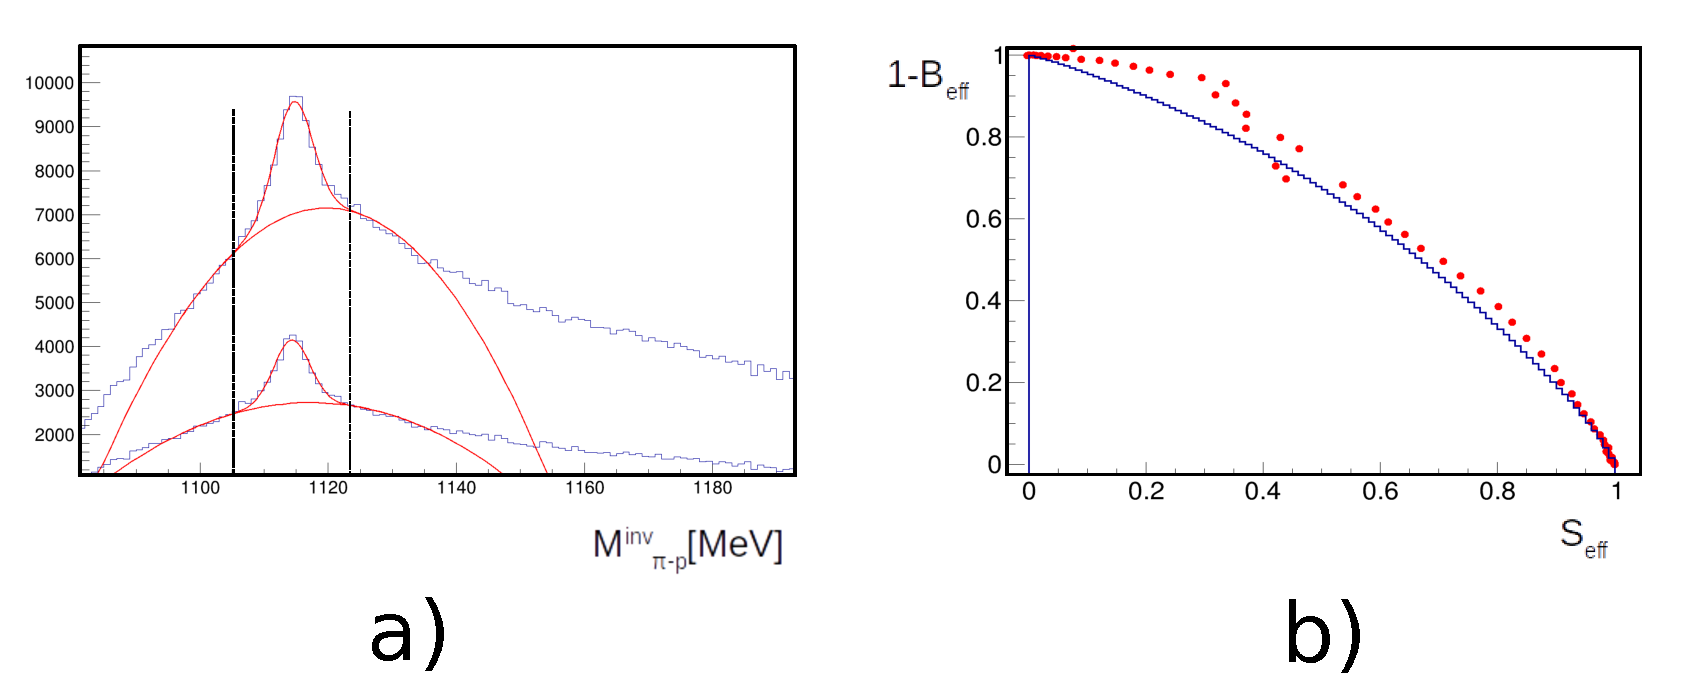
\includegraphics[width=0.9 \textwidth]{Chapter_NN/NN_wyniki.eps}
  \caption{Results of a neural network training. a)Example of two spactra after a cut on the network output. For each of the the signal (gausian function) and background (4-th order polynomial) were fitted. Such fits allows to calculate a signal efficiency $\frac{S}{S_0}$ and a background rejection $1-\frac{B}{B_0}$, where $S_0$ and $B_0$ are yelds of signal and background without any cut on a neural network output. }
  \label{fig:NN_wynik}
\end{figure}

%%% Local Variables:
%%% TeX-master: "../main"
%%% End: 